\title{Building energy simulation test - BESTEST}
% Use \titlerunning{Short Title} for an abbreviated version of your contribution title if the original one is too long
\author{Ruben Baetens and Dirk Saelens}
\authorrunning{R. Baetens, D. Saelens}
\institute{Ruben Baetens \at K.U.Leuven, Kasteelpark Arenberg 40 bus 2447, BE-3001 Leuven (Heverlee) \email{ruben.baetens@bwk.kuleuven.be}
\and Dirk Saelens \at K.U.Leuven, Kasteelpark Arenberg 40 bus 2447, BE-3001 Leuven (Heverlee) \email{dirk.saelens@bwk.kuleuven.be}}
\maketitle

\section{Introduction}

The thermal building model are \emph{validated} by comparative tests based on the \emph{Building Energy Simulation Test} (BESTEST)~\cite{Judkoff1995, Neymark2008} as developed under supervision of the International Energy Agency (IEA)~\cite{Lomas1994,Lomas1994a} and standardized as the ANSI/ASHRAE Standard 140-2007~\cite{ASHRAE140}. This standard consists of a series of specified test cases and has been developed to diagnose whole building energy simulation software. Here, output values such as the annual energy consumptions, peak loads, average and extreme room air temperatures, and some hourly data are compared to miscellaneous building energy simulation programs, e.g. BLAST, DOE2.1D, ESP-R, SERIRES / SUNCODE, S3PAS, TASE and TRNSYS. 

\subsection{Building energy simulation test cases}

Within this work, the so-called \emph{“basic test cases} are used” to \emph{validate} the building model. These test cases test the ability to model combined effects as thermal mass, solar gains and solar shading, air infiltration, internal heat gains, sunspaces and thermostat control. Three series of basic cases are tested :

\begin{enumerate}
\item Qualification cases 600 to 650 representing a set of lightweight buildings that are relatively realistic with respect to their thermal characteristics. Within this set of cases, case 600 tests the south solar transmission, case 620 tests the east and west solar transmittance and incidence, case 640 tests night setback and case 650 tests venting.
\item Qualification cases 900 to 960 representing a set of heavyweight buildings that are relatively realistic with respect to their thermal caracteristics and include a building configuration with a sunspace. Within this set of cases, case 900 tests the thermal mass and solar interaction, test 920 tests the east and west transmittance and its mass interaction, case 940 tests night set-back and its mass interaction, case 950 tests venting and its mass interaction and case 960 tests passive solar and interzonal heat transfer.
\item Free-float basic test cases 600FF, 900FF, 650FF and 950FF equaling the corresponding non-FF cases except the absence of a mechanical heating or cooling systems.
\end{enumerate}

%Add all tests on ground slabs too

\subsection{Test results}

\subsubsection{Annual heating and cooling loads}

\begin{figure}[ht]
\subfigure[Annual heating loads for the low mass and heavy mass buildings.]{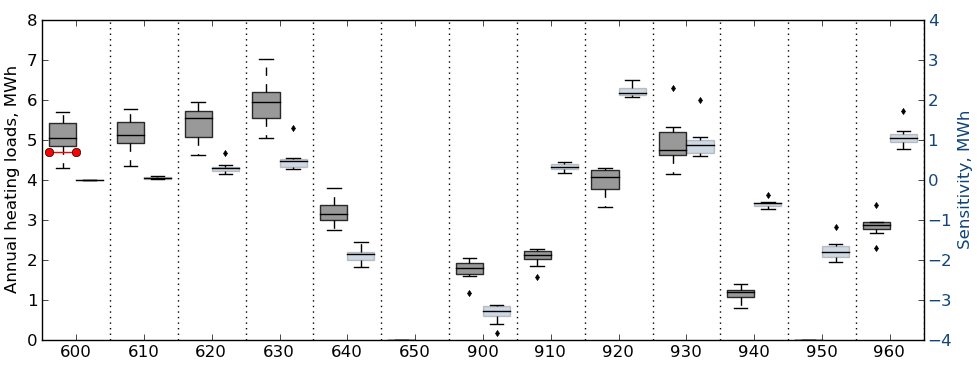
\includegraphics[width=\textwidth]{Buildings/MyGraphics/AH_BESTEST.png}\label{fig:AH_BESTEST}}
\subfigure[Annual sensible cooling loads for the low mass and heavy mass buildings.]{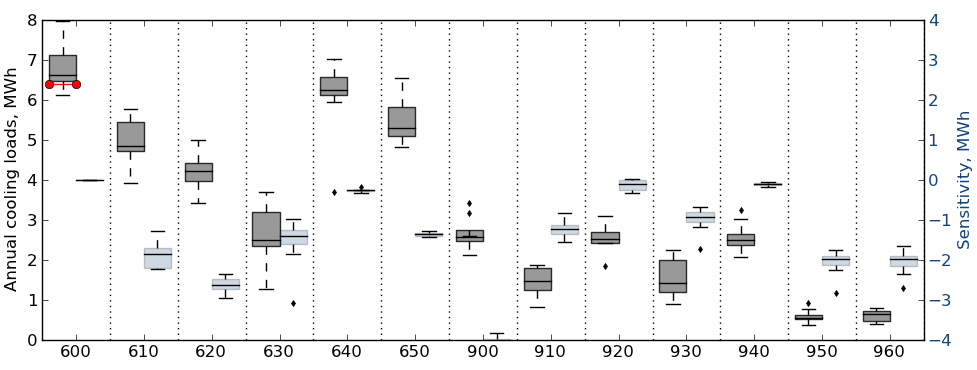
\includegraphics[width=\textwidth]{Buildings/MyGraphics/AC_BESTEST.png}\label{fig:AC_BESTEST}}
\caption{Annual heating and sensible cooling loads for the low mass and heavy mass buildings.} 
\end{figure}

\subsubsection{Peak heating and cooling loads}

\begin{figure}[t]
 \center
 \begin{tikzpicture}
\begin{axis} [
 width=12.8cm, height=4.9cm,
 xmin=-0.8, xmax=13.8,
 ymin=-0.1,  ymax=1.6,
 scatter/classes={a={darkgray,scale=0.7,opacity=0.4},b={darkgray,mark=o,scale=0.7,opacity=0.4}}, 
 xtick={0,1,2,3,4,5,6,7,8,9,10,11,12,13},
 xticklabels={\eg,600,610,620,630,640,650,900,910,920,930,940,950,195},]
 \addplot[scatter, only marks, scatter src=explicit symbolic] table [x=x,y=y1,meta=label]{./data/bestest.dat};
 \addplot[scatter, only marks, scatter src=explicit symbolic] table [x=x,y=y2,meta=label]{./data/bestest.dat};
 \addplot[scatter, only marks, scatter src=explicit symbolic] table [x=x,y=y3,meta=label]{./data/bestest.dat};
 \addplot[scatter, only marks, scatter src=explicit symbolic] table [x=x,y=y4,meta=label]{./data/bestest.dat};
 \addplot[scatter, only marks, scatter src=explicit symbolic] table [x=x,y=y5,meta=label]{./data/bestest.dat};
 \addplot[scatter, only marks, scatter src=explicit symbolic] table [x=x,y=y6,meta=label]{./data/bestest.dat};
 \addplot[scatter, only marks, scatter src=explicit symbolic] table [x=x,y=y7,meta=label]{./data/bestest.dat};
% \addplot coordinates {(-1, 0.9)(15, 0.9)};
 \addplot coordinates {(-1, 1)(15, 1)};
 %reference
 \addplot[color=black,mark=halfcircle*] coordinates {(-0.24, 1.05)(-0.08, 1.1)(0.08, 0.95)(0.24, 0.9)};
 \node[pin=90:{\footnotesize $Q_{h}$}] at (axis cs:-0.24,1.05) {};
 \node[pin=90:{\footnotesize $P_{h}$}] at (axis cs:0.08,0.95) {};
 \node[pin=-90:{\footnotesize $Q_{c}$}] at (axis cs:-0.08,1.1) {};
 \node[pin=-90:{\footnotesize $P_{c}$}] at (axis cs:0.24,0.9) {};
 \node[pin=180:{\footnotesize \textsc{bestest}}] at (axis cs:3.92,1.403) {};
 %case600
 \addplot[color=black,mark=halfcircle*] coordinates {(0.76, 1.038)(0.92, 0.972)(1.08, 0.967)(1.24, 1.029)}; %wettercorr
 %case610
 \addplot[color=black,mark=halfcircle*] coordinates {(1.76, 1.034)(1.92, 0.944)(2.08, 0.967)(2.24, 0.961)}; %wettercorr
 %case620
 \addplot[color=black,mark=halfcircle*] coordinates {(2.76, 0.987)(2.92, 0.906)(3.08, 0.952)(3.24, 0.974)}; %wettercorr
 %case630
 \addplot[color=black,mark=halfcircle*] coordinates {(3.76, 0.943)(3.92, 1.045)(4.08, 0.966)(4.24, 0.998)}; %wettercorr
 %case640
 \addplot[color=black,mark=halfcircle*] coordinates {(4.76, 1.000)(4.92, 1.078)(5.08, 1.091)(5.24, 1.036)}; %wettercorr
 %case 650
 \addplot[color=black,mark=halfcircle*] coordinates {(5.92, 1.094)(6.24, 1.048)}; %wettercorr
 %case900
 \addplot[color=black,mark=halfcircle*] coordinates {(6.76, 0.828)(6.92, 0.797)(7.08, 0.906)(7.24, 0.828)}; %wettercorr
 %case910
 \addplot[color=black,mark=halfcircle*] coordinates {(7.76, 0.792)(7.92, 0.636)(8.08, 0.862)(8.24, 0.808)}; %wettercorr
 %case920
 \addplot[color=black,mark=halfcircle*] coordinates {(8.76, 0.839)(8.92, 0.787)(9.08, 0.874)(9.24, 0.846)}; %wettercorr
 %case930
 \addplot[color=black,mark=halfcircle*] coordinates {(9.76, 0.781)(9.92, 0.906)(10.08, 0.878)(10.24, 0.884)}; %wettercorr
 %case940
 \addplot[color=black,mark=halfcircle*] coordinates {(10.76, 0.718)(10.92, 0.787)(11.08, 0.820)(11.24, 0.868)}; %wettercorr
 %case950
 \addplot[color=black,mark=halfcircle*] coordinates {(11.92, 1.023)(12.24, 0.956)}; %wettercorr
 %case195
 \addplot[color=black,mark=halfcircle*] coordinates {(12.76, 0.98)(12.92, 1.1096)(13.08, 0.9893)(13.24, 1.0692)}; %wettercorr
\end{axis}
\end{tikzpicture}
 \caption{Verification by \abb{bestest}' inter model comparison, denoting the annual heating loads $Q_{h}$, the annual cooling loads $Q_{c}$, the hourly integrated peak heating loads $P_{h}$ and hourly integrated peak cooling loads $P_{c}$ normalized by the all-code mean for the low and heavy mass base cases.}
\end{figure}

%\begin{figure}[ht]
%\subfigure[Peak heating loads for the low mass and heavy mass buildings.]{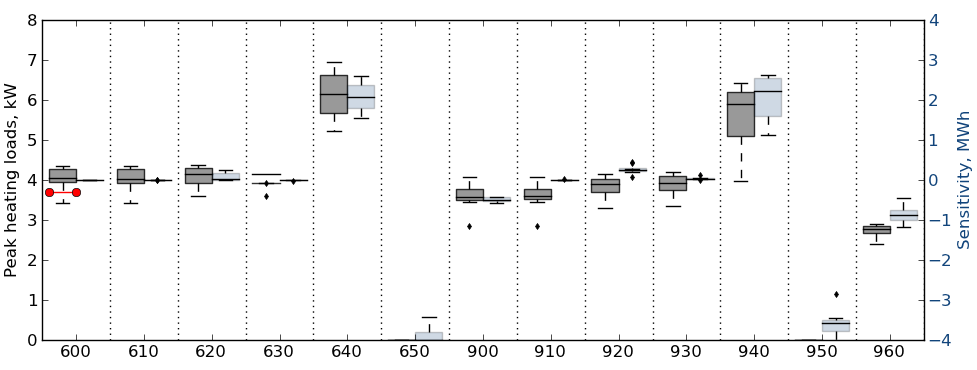
\includegraphics[width=\textwidth]{Buildings/MyGraphics/PH_BESTEST.png}\label{fig:PH_BESTEST}}
%\subfigure[Peak sensible cooling loads for the low mass and heavy mass buildings.]{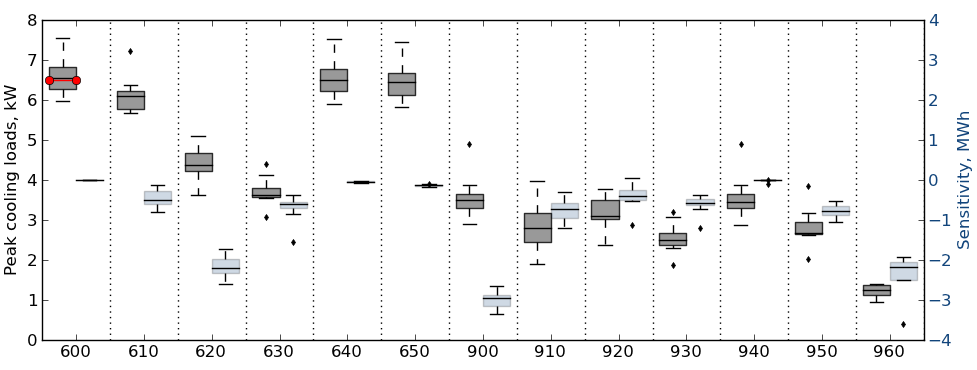
\includegraphics[width=\textwidth]{Buildings/MyGraphics/PC_BESTEST.png}\label{fig:PC_BESTEST}}
%\caption{Peak heating and sensible cooling loads for the low mass and heavy mass buildings.} 
%\end{figure}

\subsubsection{Indoor air temperatures}

\begin{figure}[ht]
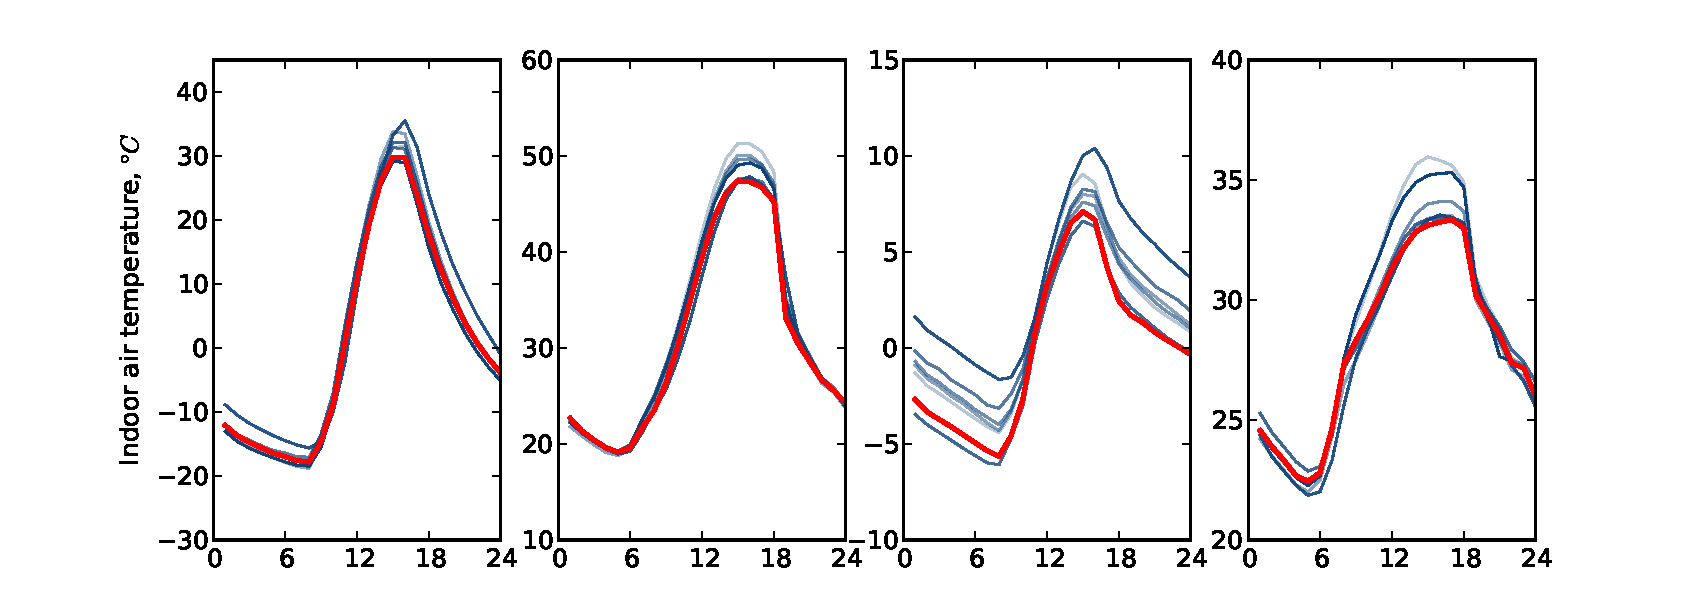
\includegraphics[width=\textwidth]{Buildings/MyGraphics/Temp_BESTEST.pdf}
\label{fig:Temp_BESTEST}
\caption{Indoor temperatures for the low mass and heavy mass buildings.} 
\end{figure}

%\bibliography{Buildings/MyBibTexLibrary}


